%!TEX root=../mythesis.tex
% Chapter Template

\chapter{Background} % Main chapter title
\chaptermark{Background}  % replace the chapter name with its abbreviated form
\label{ch:background}


In this chapter, we present background that will be necessary to elaborate on our proposed approaches later in the report.
%
First, we introduce a typical experimental setup of OpenQA along with notations that we will be using throughout the report.
%
Next, we introduce Dense Passage Retrieval (DPR)~\cite{karpukhin2020dense}, a recently published work with a novel retriever training method with the negative log-likelihood objective function and in-batch negative technique.
%
We then describe the default experimental settings used in our experiments.
%
%We then review Fusion-in-Decoder (FiD)~\cite{izacard2021leveraging}, a novel generative reader model capable of reading and aggregating information from hundreds of documents to produce answers.



\section{Notations}\label{sec:notations}
%
For OpenQA, we are given a large corpus of documents containing factual information from which we retrieve knowledge needed to perform question answering.
%
It is a common practice in the OpenQA literature to split each of these documents into several text chunks of equal lengths~\cite{karpukhin2020dense, wang2019multi, lewis2020retrieval, xiong2020approximate, fajcik2021pruning, izacard2020distilling, izacard2021leveraging}, resulting in a corpus $\mathcal{C}$ of $M$ passages $\mathcal{C} = \{p_1, p_2, \ldots, p_M\}$.
%
This is because existing reading comprehension methods have a limited capability of reading long sequences as discussed in~\sref{sec:open_book}.
%
Each passage $p_i$ can further be viewed as a sequence of tokens (words) $w_1^{(i)}, w_2^{(i)}, \ldots, w_{\vert p_i \vert}^{(i)}$.
%
Given an input question $q$, the task is to find its answer under the form of a text span $w_{s, e}^{(i)} = w_s^{(i)}, w_{s + 1}^{(i)}, \ldots, w_e^{(i)}$ of a passage $p_i$, where $s$ and $e$ denote the~\emph{start} and~\emph{end} indices of the span, respectively.
%
It is important to highlight the flexibility of OpenQA that during inference, any text corpus can be used to answer the question as long as it provides necessary information.
%
In practice, the corpus size can range from millions (e.g., Wikipedia) to billions or trillions (e.g., the Web) of passages.

%
Under the two-stage retriever-reader paradigm, we have a retriever $R$ and a reader $S$ formulated as
%
\begin{definition}[Retriever]
	A retriever under the two-stage paradigm is a model that returns a small filtered subset of the given large set of passages.
	\begin{equation}
	R(q, \mathcal{C}) = \mathcal{C_F}
	\end{equation}
\end{definition}
%
\begin{definition}[Reader]
	A reader under the two-stage paradigm is a model that produces an answer to the given question given the filtered set from the retriever.
	\begin{equation}
	S(q, \mathcal{C_F}) = w_{s, e}^{(i)}
	\end{equation}
\end{definition}
%
where $\mathcal{C_F}$ is a small set of $k$ passages with $k \ll M$ and $w_{s, e}^{(i)}$ is the final answer of the OpenQA system to the question $q$.
%
In other words, the task of the retriever is to efficiently retrieve a small set $\mathcal{C_F}$ of passages that it considers relevant.
%
The reader will then carefully comprehend the question $q$ as well as each of the passages in $\mathcal{C_F}$ to infer the answer.
%
We refer readers to~\fref{fig:open_book_openqa} for an illustration of an OpenQA system.

Furthermore, throughout this report, we refer to an~\emph{encoder}, denoted as $E$, as a BERT model~\cite{devlin2019bert} that first appends a special token \texttt{[CLS]} to the input text sequence and then maps the sequence to the embedding of \texttt{[CLS]}.
\begin{definition}[Encoder]
	An encoder is a model that maps an input text sequence
	\begin{align*}
	p = \{\texttt{[CLS]}, w_1, w_2, \ldots, w_{\vert p \vert}\}
	\end{align*}
	to the vector embedding of the special token token $\texttt{[CLS]}$
	\begin{equation}
	E(p)_{\texttt{[CLS]}} = \mathbf{v}_{\texttt{[CLS]}} \in \mathbb{R}^{d}
	\end{equation}
\end{definition}
%
where $d$ is the embedding dimension, and $\mathbf{v}_{\texttt{[CLS]}}$ is known as the feature representation~\footnote{In this report we will use~\emph{embedding},~\emph{feature} and~\emph{representation} interchangeably.} of the special token \texttt{[CLS]}.
%
Historically, \texttt{[CLS]} is appended to the input to serve as a contextualized embedding that encodes the semantic meaning of the \emph{entire} sequence~\cite{devlin2019bert}.
%
With a proper objective function, we can train $E$ to encode important semantic meaning of $p$ into $\mathbf{v}_{\texttt{[CLS]}}$.




\section{DPR Retriever}
\label{sec:dpr_retriever}


\begin{figure}[!htbp]
	\centering
	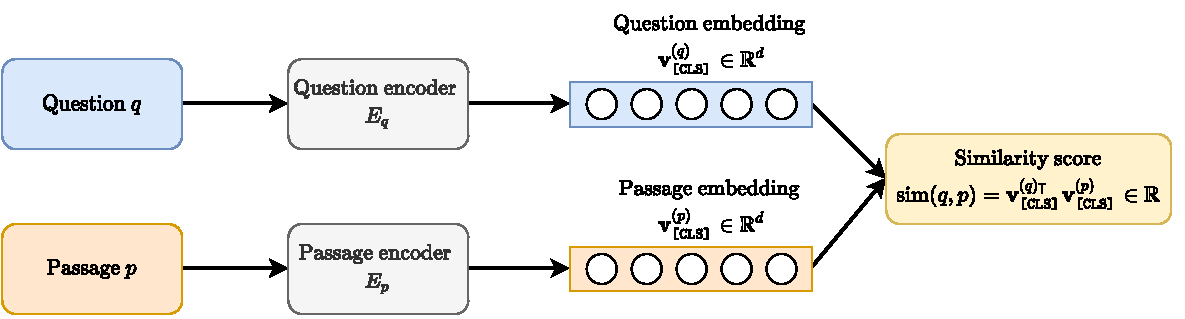
\includegraphics[width=0.9\linewidth]{background/two_tower.pdf}
	\caption[Two-tower architecture of DPR retriever.]{
		%
		The two-tower architecture of the DPR retriever, consisting of a question encoder and a passage encoder.
		%
		Each of the towers encodes input texts into their embedding vectors, and the final similarity score is computed as their dot product.
		%
		Adapted from~\cite{chen2020open}.
	}
	\label{fig:two_tower}
\end{figure}


%
Despite its simplicity, DPR was able to outperform all prior arts by large margins when it was introduced.
%
In this section, we describe the retriever component of DPR and refer interested readers to~\cite{karpukhin2020dense} for a detailed description of the reader component.
%
The DPR retriever consists of a passage encoder $E_P$ and a question encoder $E_Q$, whose task is to embed passages and questions to their representation space, respectively.
%
\begin{equation}
	\label{eq:dpr_encode}
	\begin{split}
	E_P(p)_{\texttt{[CLS]}} = \mathbf{v}^{(p)}_{\texttt{[CLS]}} \in \mathbb{R}^d \\ 
	E_Q(q)_{\texttt{[CLS]}} = \mathbf{v}^{(q)}_{\texttt{[CLS]}} \in \mathbb{R}^d
	\end{split}
\end{equation}
%
We then define the similarity between a question and a passage as their dot product.
\begin{definition}[Vector similarity]
	\label{def:sim}
	The similarity between a question and a passage is defined as the dot product of their vector embeddings.
	\begin{equation}
	\label{eq:sim_score}
	\text{sim}(q, p) = \mathbf{v}^{(q)\intercal}_{\texttt{[CLS]}} \mathbf{v}^{(p)}_{\texttt{[CLS]}} \in \mathbb{R}
	\end{equation}
\end{definition}
%
\fref{fig:two_tower} presents an illustration of the DPR retriever.
%
This two-tower architecture is widely used in~\emph{metric learning}~\cite{han2015matchnet, song2019occlusion} and~\emph{self-supervised learning}~\cite{zbontar2021barlow, mitrovic2020representation} in which models are trained to maximize the similarity of similar inputs and minimize the similarity of dissimilar inputs.
%
As discussed in~\sref{sec:open_book}, this design brings about the real-time performance of the well-studied Maximum Inner Product Search (MIPS) algorithm~\cite{johnson2019billion} but at the same time is detrimental to the retrieval performance due to the decomposability gap which we aim to address.

%
In this project, we follow the DPR implementation and use BERT~\cite{devlin2019bert} as the architecture for all encoders.
%
As a result, each embedding vector is a $d=768$-dimensional vector.
%
We omit the details of BERT and refer interested readers to~\cite{devlin2019bert}.

%
\subsection{Training and Inference}
\label{sec:dpr_training}
%
Given an input question $q_i$ posed by users, we denote $p^{+}_i$ as a positive passage that contains an answer to $q_i$, and $p^{-}_i$ as a negative passage otherwise.
%
Intuitively, we want to train the model to maximize the similarity between $q_i$ and $p^{+}_i$, at the same time minimizing the similarity between $q_i$ and $p^{-}_i$.
%
Formally, under the metric learning framework, we want to construct an \emph{latent space} such that relevant pairs of questions and passages are closer to each other than irrelevant pairs.
%
Therefore, given a question $q_i$, a relevant passage $p^{+}_i$ and a set of $n$ irrelevant passages $\{p^{-}_{i, 1}, p^{-}_{i, 2}, \ldots, p^{-}_{i, n}\}$, we train the model to minimize the negative log-likelihood loss function:
%
\begin{definition}[Negative log-likelihood]
	\label{def:nll}
	The negative log-likelihood loss function of the positive passages.
	\begin{equation}
	L(q_i, p^{+}_i, p^{-}_{i, 1}, p^{-}_{i, 2}, \ldots, p^{-}_{i, n}) = - \log \frac{e^{\text{sim}(q_i, p^{+}_i)}}{e^{\text{sim}(q_i, p^{+}_i)} + \sum_{j = 1}^{n} e^{\text{sim}(q_i, p^{-}_{i, j})}}
	\end{equation}
\end{definition}
%
where we apply the softmax function to the similarity vector before taking its negative log value.
\begin{definition}[Softmax]
	\label{def:softmax}
	Softmax is the function that takes as input a vector of $K$ real numbers and outputs a normalized probability distribution vector of the same length.
	\begin{equation}
	\sigma(\mathbf{z})_i = \frac{e^{z_i}}{\sum_{j = 1}^{K}e^{z_j}} \text{ for } i = 1, 2, \ldots, K
	\end{equation}
\end{definition}
%
In practice, we consider passages to be positive if they contain a text span that matches the answer of the question, and negative otherwise.

%
In addition to the simple yet novel negative log-likelihood objective function,~\citet{karpukhin2020dense} also proposed a simple in-batch negative training setting that works extremely well empirically.
%
Suppose we have a mini-batch of $B$ (question, positive passage) pairs.
%
We first feed this batch through the two-tower retriever to obtain a question embedding matrix $\mathbf{Q} \in \mathbb{R}^{B \times d}$ and a passage embedding matrix $\mathbf{P} \in \mathbb{R}^{B \times d}$.
%
The similarity matrix is then computed as:
%
\begin{equation}
\mathbf{S} = \mathbf{Q}\mathbf{P}^\intercal \in \mathbb{R}^{B \times B}
\end{equation}
%
By doing so, we are effectively comparing $B^2$ question-passage pairs in the mini-batch, from which we want to minimize the negative log of the softmaxed values along the diagonal of the square similarity matrix $\mathbf{S}$.
%
This is called~\emph{in-batch negatives} since we reuse computations from within the batch with positive passages of other questions as negative passages, thereby efficiently reducing the memory footprint and effectively scaling the batch size up.
%
Furthermore,~\citet{karpukhin2020dense} proposed to utilize an additional hard negative passage per each question in the minibatch, obtained from the sparse retrieval method BM25~\cite{robertson2009probabilistic}.
%
In other words, each question will be associated with a single positive passage and $2B - 1$ negative passages, of which $2(B - 1)$ passages are in-batch negatives and one passage is hard negative.

%
During inference, we first build a FAISS index~\cite{johnson2019billion} by feeding all available passages in the corpus to $E_P$.
%
This incurs a non-recurring cost since this step is only done once.
%
At run-time, given an input question $q$, we obtain its embedding via $\mathbf{v}^{(q)}_{\texttt{[CLS]}} = E_Q(q)_{\texttt{[CLS]}}$, which gets sent to the FAISS index to perform top-$k$ similarity search.
%
A set $\mathcal{C_F}$ of top-$k$ most relevant passages according to the similarity score $\text{sim}(q, p_i)$ is produced by the algorithm in milliseconds, concluding the retrieval step.



\section{Experimental Setup}\label{sec:exp_setup}
%
In this section we briefly describe the default experimental setup used in our experiments.
%
We note that we reuse a substantial portion of the code and data given by the DPR authors~\footnote{https://github.com/facebookresearch/DPR/}~\cite{karpukhin2020dense}, unless otherwise specified below.
%
Therefore, we refer interested readers to~\cite{karpukhin2020dense} for further details on the setup.

\subsection{Data}\label{sec:exp_data}
%
Following~\cite{karpukhin2020dense}, we use the English Wikipedia dump from Dec. 20, 2018 as the knowledge source from which passage retrieval is done.
%
This knowledge base is provided by the DPR authors after post-processed to remove semi-structured data and split into chunks of 100-word passages.
%
There are in total 21,015,324 passages in this corpus.
%
On the other hand, we use Natural Questions (NQ)~\cite{kwiatkowski2019natural} as the question answering dataset on which we train and evaluate our retriever and reader models.
%
This dataset provides questions mined from the real Google search queries as well as the corresponding positive Wikipedia passages along with the answer text span.

\subsection{Evaluation Metrics}
%
Following~\cite{karpukhin2020dense}, we evaluate the retriever model by the~\emph{retrieval accuracy} and the reader model with~\emph{exact match (EM)} and~\emph{F1 score}.
%
Specifically, retrieval accuracy, or retrieval recall, is measured as the percentage of top-$k$ retrieved passages that contain the gold answer obtained from NQ.
%
It can be understood as how relevant your retrieved passages are to a given question.
%
On the reader side, exact match is a direct measure of the reader model performance.
%
It is calculated as the percentage of answers returned by the reader model that precisely match with one of the gold answers.
%
F1 score on the other hand allows some relexations on the returned answers by measuring the F1 score between the answer by the reader model and the gold answer.
%
\begin{definition}[F1 score]
	F1 score in the context of QA is calculated as the harmonic mean between the precision and recall of the returned answer and the gold answer.
	\begin{equation}
	\label{eq:f1_score}
	F_1 = \frac{2}{\text{recall}^{-1} + \text{precision}^{-1}}
	\end{equation}
\end{definition}